\section{GPU Collector Integration}
\label{sec:gpu_collector}
\subsection{Introduction and Motivation}
\label{subsec:gpu_intro}

Accelerators are increasingly responsible for the energy footprint of modern
compute workloads.  
To attribute this consumption to containerized applications with high temporal
accuracy, Tycho must incorporate GPU telemetry into the same unified timing
model used for RAPL, eBPF, and Redfish domains
(\S~\ref{sec:tycho_timing_engine}).  
Achieving this integration is challenging: GPU drivers do not expose continuous
measurements but publish telemetry at discrete, hardware-dependent intervals.
If these intervals are not respected, sampling quickly suffers from aliasing,
redundant reads, and temporal drift across subsystems, as well as imprecise timing.

NVIDIA’s telemetry interfaces further complicate accurate measurement.  
The widely used \code{nvmlDeviceGetPowerUsage} function reports a
\emph{one-second trailing average}\parencite{nvidia_nvml_api}, not the instantaneous power required for
sub-second energy attribution.  
High-frequency power samples are available only through specialised field APIs.
Cumulative energy counters (when present) provide authoritative publish
boundaries, but they are absent on many devices, including consumer GPUs and
MIG configurations.  
Process-level telemetry is even more restrictive: NVML aggregates utilisation
over caller-specified wall-clock windows and provides no information about the
device’s internal publish cadence.

Because of these structural limitations, fixed polling intervals or naïve
periodic sampling are fundamentally insufficient.  
Accurate attribution requires that Tycho (i) infer the GPU’s implicit publish
cadence, (ii) align its sampling with this cadence, and (iii) integrate both
device- and process-level telemetry into the global measurement timeline without
violating the strict monotonic ordering enforced by Tycho’s multi-domain ring
buffer (\S~\ref{subsec:ringbuffer_overview}).

This work introduces two contributions that address these challenges:

\begin{itemize}
  \item \textbf{A phase-aware sampling mechanism} that infers the GPU’s hidden
  publish rhythm and adaptively concentrates polling around predicted update
  edges.  
  This transforms GPU sampling from periodic polling into a timing-aligned,
  event-driven process.

  \item \textbf{A unified integration of GPU telemetry} into Tycho’s global
  timebase, producing exactly one \code{GpuTick} per confirmed hardware update,
  with timestamps that are directly comparable to all other energy domains.
\end{itemize}

Together, these mechanisms provide temporally precise, low-latency GPU
measurements while respecting the variability and constraints of NVIDIA’s
telemetry ecosystem.  
This elevates the GPU subsystem to a first-class energy domain in Tycho and
enables accurate container-level attribution in heterogeneous accelerator
environments.


\subsection{Architectural Overview}
\label{subsec:gpu_architecture}

The GPU collector is organised as a layered subsystem that integrates vendor
telemetry, adaptive timing, and unified buffering into a coherent measurement
pipeline.  
Its structure reflects Tycho’s core design principles: strict adherence to a
monotonic timebase, decoupling of heterogeneous sampling frequencies, and
event-driven integration into the platform-wide timing and buffering
infrastructure (\S~\ref{sec:tycho_timing_engine},
\S~\ref{subsec:ringbuffer_overview}).

At the lowest layer, the collector interfaces with NVIDIA accelerators through a
backend abstraction compatible with both \code{NVML} and \code{DCGM} ("\textit{Data Center GPU Manager}").  
This abstraction handles device enumeration, capability probing, MIG topology
inspection, and access to device and process telemetry.  
The collector does not assume uniform backend capabilities: cumulative energy
counters, instantaneous power fields, and process-level utilisation may or may
not be available depending on hardware generation and configuration.

Above this backend, the collector exposes two measurement paths:

\begin{itemize}
  \item \textbf{Device path.}  
  Retrieves power, utilisation, frequency, thermal, and memory metrics for all
  devices and MIG instances.  
  These values describe the instantaneous operational state of the accelerator.

  \item \textbf{Process path.}  
  Aggregates per-process utilisation over a backend-defined wall-clock window.  
  This enables multi-tenant attribution but is inherently retrospective and
  independent of the device’s internal publish cadence.
\end{itemize}

Both paths feed into a shared sampling layer governed by Tycho’s timing engine.  
The device path is triggered by a \emph{phase-aware scheduler} that aligns its
polling activity with the driver’s implicit publish cadence.  
The process path is invoked only when a device update is detected, ensuring
temporal alignment between instantaneous device measurements and aggregated
process data.

The final integration step mirrors all other Tycho subsystems:  
each confirmed hardware update is converted into a \code{GpuTick} structure
containing device and (optionally) process snapshots, together with a strictly
ordered monotonic timestamp.  
This tick is emitted into Tycho’s multi-domain ring buffer, where it becomes
part of the unified energy timeline used for correlation and attribution across
eBPF, RAPL, and platform power domains.

Figure~\ref{fig:gpu_phaseaware_timeline} (later in this section) provides a
conceptual overview of this pipeline, illustrating the interaction between the
backend interface, the phase-aware sampler, and Tycho’s global collection
engine.


\subsection{Phase-Aware Sampling: Conceptual Overview}
\label{subsec:gpu_phaseaware_concept}

GPU drivers publish power and utilisation metrics at discrete, device-internal
intervals.  
These updates occur neither continuously nor synchronously with the sampling
frequencies required by Tycho’s timing engine.  
Because the driver does not expose its publish cadence directly, a naïve
fixed-interval polling strategy risks both \emph{aliasing} (missing updates) and
\emph{redundancy} (repeatedly reading identical values).  
Either effect would distort the temporal alignment of GPU measurements with the
rest of Tycho’s energy domains.

To avoid this, the GPU collector introduces a \emph{phase-aware sampling}
mechanism that infers the driver’s implicit publish cadence from observations.  
The sampler tracks two quantities: an estimated publish period and the phase
offset between the device’s update rhythm and Tycho’s monotonic timebase.  
By predicting the next likely update moment, the sampler can modulate its
polling intensity accordingly:  

\begin{itemize}
  \item \textbf{Base mode:} low-frequency polling maintains coarse alignment and
  detects long-term drift in the publish cadence.

  \item \textbf{Burst mode:} when the current time approaches a predicted update
  edge, the sampler briefly increases its polling frequency to minimise the
  latency between the hardware update and Tycho’s observation of it.
\end{itemize}

This adaptive strategy ensures that Tycho reads the device only when a fresh
publish is likely to be available.  
Freshness is determined by comparing each snapshot to the most recent confirmed
update, preferably via cumulative energy counters when present, or otherwise via
power deltas exceeding a configurable threshold.  
Only when a new publish is detected does the sampler emit an event.

The resulting behaviour is simple but powerful:
\begin{quote}
\emph{Each hardware update produces exactly one \code{GpuTick}, and no tick is
emitted unless the device has genuinely updated.}
\end{quote}
This one-to-one correspondence is critical for integrating GPU measurements into
Tycho’s unified energy timeline.  
It guarantees temporal fidelity, eliminates redundant samples, and ensures that
GPU metrics are directly comparable with other measurements
obtained under the same timing and buffering semantics.

The next subsection formalises this behaviour by presenting the timing model
used to estimate publish periods, track phase offsets, and define the burst
window around predicted update edges.


\subsection{Phase-Aware Timing Model}
\label{subsec:gpu_phaseaware_math}

The timing model enables Tycho to infer the GPU driver's implicit publish
cadence and to align sampling with the actual update moments of the hardware.
It maintains two quantities derived from confirmed device updates:
an estimate of the \emph{publish period} and a \emph{phase offset} relative to
Tycho's monotonic clock.  
This subsection presents the model in a unified mathematical form.

Let $t_{\text{obs},k}$ denote the monotonic timestamp of the $k$-th confirmed
hardware update.  
From these observations, the sampler derives the period estimate $\hat{T}_k$
and phase estimate $\hat{\phi}_k$.

\paragraph{Period Estimation.}
Each new inter-update interval
\[
  \Delta t_k = t_{\text{obs},k} - t_{\text{obs},k-1}
\]
provides a direct sample of the device's publish period.  
To remain robust to jitter caused by DVFS, thermal transitions, or backend
noise, the sampler applies an exponential moving average (EMA):
\[
  \hat{T}_k = (1 - \alpha_T)\,\hat{T}_{k-1} + \alpha_T\,\Delta t_k,
\]
with $\alpha_T \in (0,1)$ controlling the smoothing strength.  
The resulting estimate is clamped to a stable range derived from Tycho’s engine
cadence, ensuring predictable behaviour across different GPUs.

\paragraph{Phase Tracking.}
Given a current period estimate, the expected time of the $k$-th update is
\[
  \hat{t}_k = t_{\text{obs},k-1} + \hat{\phi}_{k-1} + \hat{T}_k.
\]
The deviation
\[
  \delta_k = t_{\text{obs},k} - \hat{t}_k
\]
represents the phase error.  
The sampler updates its phase estimate through a second EMA:
\[
  \hat{\phi}_k = (\hat{\phi}_{k-1} + \alpha_\phi\,\delta_k)
  \bmod \hat{T}_k,
\]
where $\alpha_\phi$ is a small adaptation constant.
This ensures smooth convergence toward the device’s true publish rhythm.

\paragraph{Edge Prediction.}
At an arbitrary time $t_{\text{now}}$, the predicted next update edge is
\[
  t_{\text{next}}
  = t_{\text{obs},k}
  + n\cdot \hat{T}_{k+1}
  + \hat{\phi}_{k+1},
\]
where $n$ is the smallest non-negative integer such that
$t_{\text{next}} \ge t_{\text{now}}$.  
This prediction determines where sampling effort should be concentrated.

\paragraph{Burst Window.}
To avoid continuous high-frequency polling, the sampler restricts hyperpolling
to a narrow window of half-width $w$ around $t_{\text{next}}$:
\[
  \text{mode}(t_{\text{now}}) =
  \begin{cases}
    \text{burst}, & |t_{\text{now}} - t_{\text{next}}| \le w, \\
    \text{base},  & \text{otherwise}.
  \end{cases}
\]
The width $w$ is expressed as a fraction of the calibrated engine cadence,
ensuring proportional behaviour across platforms.

\paragraph{Summary.}
The phase-aware model enables Tycho to infer the GPU's implicit publish cadence
solely from observed updates and to align sampling with the device’s true update
edges.  
By combining smooth period estimation, adaptive phase correction, and narrow
burst windows around predicted publishes, the sampler detects new hardware
updates with low latency and emits exactly one \code{GpuTick} per publish.

Figure~\ref{fig:gpu_phaseaware_timeline} visualises the behaviour of the
phase-aware sampling model introduced above.  
The top lane represents the hardware’s implicit publish sequence; the middle lane
shows Tycho’s adaptive polling pattern during both calibration and the
phase-locked regime; and the bottom lane shows the resulting GPU ticks,
demonstrating the one-to-one mapping between fresh device updates and emitted
\code{GpuTick} events.

\begin{figure}[H]
\centering
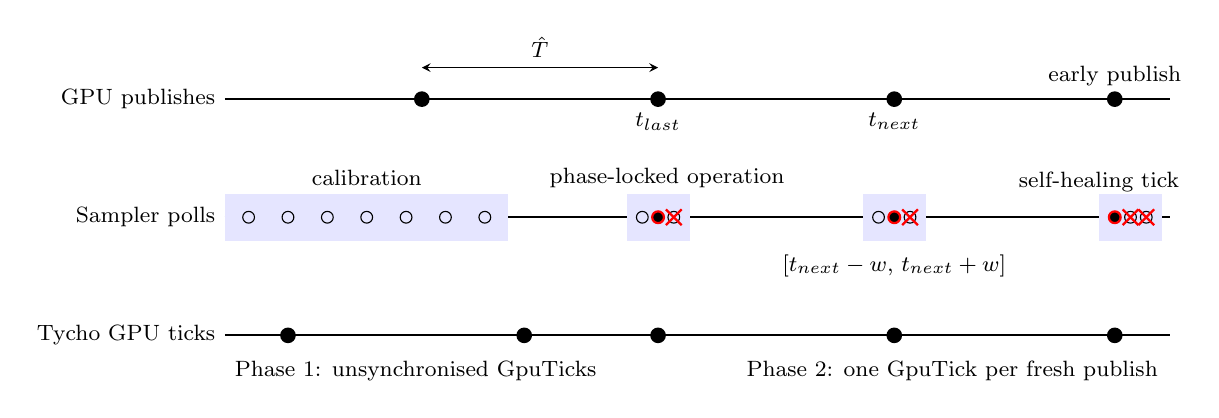
\begin{tikzpicture}[
    >=stealth,
    publish/.style={circle,fill=black,inner sep=2pt},
    poll-calib/.style={circle,draw=black,inner sep=1.5pt},
    poll-base/.style={circle,fill=black,inner sep=1.5pt},
    poll-burst/.style={circle,draw=black,inner sep=1.5pt},
    tick/.style={circle,fill=black,inner sep=2pt},
    timeline/.style={thick},
    label/.style={font=\footnotesize}
]

% Horizontal extents
\def\xmin{0}
\def\xmax{12}

% Y positions for the three lanes
\def\ygpu{3.2}
\def\ysampler{1.7}
\def\ytick{0.2}

% ------------------------------------------------------------------
% 1) GPU publish lane (ground truth)
% ------------------------------------------------------------------
\draw[timeline] (\xmin,\ygpu) -- (\xmax,\ygpu);
\node[label,anchor=east] at (\xmin,\ygpu) {GPU publishes};

% True publish events (roughly equidistant)
\foreach \x in {2.5,5.5,8.5,11.3} {
  \node[publish] at (\x,\ygpu) {};
}
\node[label,anchor=south] at (11.3,\ygpu+0.05) {early publish};

% Annotate approximate period between two publishes
\draw[<->] (2.5,\ygpu+0.4) -- node[label,above] {$\hat{T}$} (5.5,\ygpu+0.4);

% Mark t_last and t_next for illustration
\node[label,anchor=north] at (5.5,\ygpu-0.05) {$t_{\text{last}}$};
\node[label,anchor=north] at (8.5,\ygpu-0.05) {$t_{\text{next}}$};

% ------------------------------------------------------------------
% 2) Sampler lane (calibration + phase-locked polls with burst window)
% ------------------------------------------------------------------
\draw[timeline] (\xmin,\ysampler) -- (\xmax,\ysampler);
\node[label,anchor=east] at (\xmin,\ysampler) {Sampler polls};

% Calibration phase block (left)
\def\xcalibStart{0.0}
\def\xcalibEnd{3.6}
\fill[blue!10] (\xcalibStart,\ysampler-0.3) rectangle (\xcalibEnd,\ysampler+0.3);
\node[label] at ({0.5*(\xcalibStart+\xcalibEnd)},\ysampler+0.50) {calibration};

% Calibration-phase polls (irregular, more frequent)
\foreach \x in {0.3,0.8,1.3,1.8,2.3,2.8,3.3} {
  \node[poll-calib] at (\x,\ysampler) {};
}

% Burst-style windows around predicted publish times in phase-locked regime
\def\tpred{5.5}
\def\whalf{0.4}
\fill[blue!10] (\tpred-\whalf,\ysampler-0.3) rectangle (\tpred+\whalf,\ysampler+0.3);

\def\tpred{8.5}
\def\whalf{0.4}
\fill[blue!10] (\tpred-\whalf,\ysampler-0.3) rectangle (\tpred+\whalf,\ysampler+0.3);
\node[label,anchor=north] at (\tpred,\ysampler-0.35)
  {$[t_{\text{next}}-w,\,t_{\text{next}}+w]$};

\def\tpred{11.5}
\def\whalf{0.4}
\fill[blue!10] (\tpred-\whalf,\ysampler-0.3) rectangle (\tpred+\whalf,\ysampler+0.3);

% Phase-locked base polls: successful observation polls
\node[poll-base,draw=red,thick] at (5.5,\ysampler) {};
\node[poll-base,draw=red,thick] at (8.5,\ysampler) {};
% Last window: successful observation comes slightly early
\node[poll-base,draw=red,thick] at (11.3,\ysampler) {};
\node[label,anchor=south] at (11.1,\ysampler+0.2) {self-healing tick};

% Additional burst-mode polls around t_next (denser sampling inside window)
\foreach \x in {5.3,5.7,8.3,8.7,11.5,11.7} {
  \node[poll-burst] at (\x,\ysampler) {};
}

% Polls that get skipped AFTER a successful observation:
% - in the first two windows: the late burst poll
% - in the last window: the scheduled base poll at 11.5 and the late burst poll at 11.7
\foreach \x in {5.7,8.7,11.5,11.7} {
  \draw[red,thick] (\x-0.10,\ysampler-0.10) -- (\x+0.10,\ysampler+0.10);
  \draw[red,thick] (\x-0.10,\ysampler+0.10) -- (\x+0.10,\ysampler-0.10);
}

% Optional annotation: phase-locked region
\node[label,anchor=west] at (4.0,\ysampler+0.50) {phase-locked operation};

% ------------------------------------------------------------------
% 3) Tycho GPU tick lane (two phases)
% ------------------------------------------------------------------
\draw[timeline] (\xmin,\ytick) -- (\xmax,\ytick);
\node[label,anchor=east] at (\xmin,\ytick) {Tycho GPU ticks};

% Phase 1: same cadence as publishes, but not phase-aligned (during calibration)
\foreach \x in {0.8,3.8} {
  \node[tick] at (\x,\ytick) {};
}

% Phase 2: phase-locked, one tick per fresh device update
\foreach \x in {5.5,8.5,11.3} {
  \node[tick] at (\x,\ytick) {};
}

\node[label,anchor=west] at (0.0,\ytick-0.45)
  {Phase 1: unsynchronised \code{GpuTick}s};

\node[label,anchor=west] at (6.5,\ytick-0.45)
  {Phase 2: one \code{GpuTick} per fresh publish};

\end{tikzpicture}
\caption{Phase-aware GPU polling timeline}
\label{fig:gpu_phaseaware_timeline}
\end{figure}

\subsection{Event Lifecycle}
\label{subsec:gpu_event_lifecycle}

The GPU collector converts each confirmed hardware update into a
monotonically-timestamped \code{GpuTick} that integrates into Tycho’s
multi-domain energy timeline.  
The lifecycle consists of five stages: polling, device acquisition, optional
process acquisition, freshness detection, and tick emission.

\paragraph{1.\ Poll Initiation.}
Polling is triggered solely by the phase-aware scheduler
(\S~\ref{subsec:gpu_phaseaware_concept},
\S~\ref{subsec:gpu_phaseaware_math}).  
Base-mode polls track long-term cadence drift; burst-mode polls densely probe
the vicinity of predicted update edges.  
Each poll receives a monotonic timestamp $t_{\text{now}}$ that anchors the
resulting event.

\paragraph{2.\ Device Snapshot Acquisition.}
A poll retrieves device-level telemetry for all GPUs and MIG instances,
capturing power, utilisation, clocks, thermals, and memory state.  
All values reflect the device’s instantaneous condition at $t_{\text{now}}$ and
form a consistent cross-device snapshot of the accelerator subsystem.

\paragraph{3.\ Optional Process Snapshot Acquisition.}
If available, process-level telemetry is sampled over a backend-defined
wall-clock window (\S~\ref{subsec:gpu_process_window}).  
Although retrospective, these samples are associated with the same monotonic
timestamp as the device snapshot, ensuring that device and process data remain
correlated without temporal ambiguity.

\paragraph{4.\ Freshness Determination.}
The collector compares the new device snapshot with the most recent confirmed
update.  
Cumulative energy counters, when available, serve as the authoritative freshness
signal; otherwise Tycho uses a power-delta threshold to avoid counting noise as
updates.  
Only fresh snapshots update the period and phase estimators and proceed to the
next stage.

\paragraph{5.\ Tick Emission.}
A fresh observation is converted into a \code{GpuTick} containing device and
(optional) process snapshots and the timestamp $t_{\text{now}}$.  
The tick is then delivered to Tycho’s multi-domain ring buffer
(\S~\ref{subsec:ringbuffer_overview}).  
If no fresh update is detected, the poll produces no tick, ensuring that the GPU
timeline faithfully reflects the hardware’s publish cadence.

\paragraph{Summary.}
The event lifecycle ensures that GPU telemetry is sampled only when meaningful,
timestamped consistently with Tycho’s timebase, and integrated without blocking
or duplication.  
Each hardware update generates exactly one \code{GpuTick}, providing a precise,
causally ordered input to Tycho’s cross-domain energy attribution pipeline.

\subsection{Per-Process Telemetry Window}
\label{subsec:gpu_process_window}

Device-level metrics describe the instantaneous state of each GPU, but many
applications require attributing accelerator activity to individual processes or
containers.  
NVIDIA’s interfaces provide such information only in the form of \emph{aggregated
utilisation over a caller-specified time window}.  
Correctly selecting and interpreting this window is essential for obtaining
meaningful per-process data and for aligning process-level records with the
device-level timeline maintained by Tycho.

\paragraph{Wall-Clock Semantics.}
Unlike device publishes, which occur on the GPU’s internal cadence,
NVIDIA’s per-process APIs integrate utilisation over a duration supplied by the
caller.  
These interfaces expect a \emph{wall-clock} interval, expressed in milliseconds,
rather than a duration derived from Tycho’s monotonic timebase.  
The distinction is crucial: Tycho’s monotonic clock operates on an internal
quantum chosen to support high-resolution scheduling (\S~\ref{sec:tycho_timing_engine}),
but this quantum has no defined relationship to real elapsed time.  
Using monotonic differences directly would produce windows that are several
orders of magnitude too short, yielding incomplete utilisation samples.

For this reason, Tycho maintains a separate wall-clock origin for each GPU or
MIG instance.  
Whenever process telemetry is requested, the duration since the last successful
query is computed using wall-clock time, ensuring that the backend receives a
true real-time interval.

\paragraph{Window Derivation.}
For each owner (physical GPU or MIG instance), Tycho records the timestamp
$t^{(i)}_{\text{last}}$ of the most recent successful process query.  
When a new query occurs at time $t^{(i)}_{\text{now}}$, the raw duration
\[
  \Delta t^{(i)}_{\text{raw}} = t^{(i)}_{\text{now}} - t^{(i)}_{\text{last}}
\]
is transformed according to backend expectations:

\begin{enumerate}
  \item \emph{Clamping.}  
  The duration is restricted to a safe range  
  $\Delta t_{\min} \le \Delta t^{(i)} \le \Delta t_{\max}$  
  to avoid zero-length or excessively long sampling windows.  

  \item \emph{Millisecond granularity.}  
  NVIDIA’s process APIs accept durations in whole milliseconds.  
  Tycho therefore rounds the clamped value up to the next full millisecond to
  prevent systematic underestimation of utilisation.
\end{enumerate}

After a successful query, the wall-clock origin is updated to
$t^{(i)}_{\text{last}} \leftarrow t^{(i)}_{\text{now}}$, establishing continuity
across successive sampling windows.

\paragraph{Temporal Alignment with Device Updates.}
Even though per-process telemetry describes accumulated activity rather than a
snapshot, Tycho ensures that all process samples remain aligned with the device
timeline.  
Each process record is associated with the device-level timestamp of the poll
that triggered the query.  
If a device has never produced a fresh update, the collector uses the timestamp
of the most recent device tick as the initial origin for its process window.
This guarantees that device and process metrics are linked to the same global
temporal reference and can be fused without interpolation.

\paragraph{Backend Variability and Robustness.}
Process-level support varies widely across NVIDIA hardware and software stacks.
DCGM-capable systems typically expose high-quality, high-resolution utilisation
data, whereas NVML-only systems (particularly consumer GPUs) may provide limited
or noisy information.  
Tycho’s design accommodates these differences gracefully: when a process query
fails, the wall-clock origin is still advanced to prevent tight retry loops, and
device-level sampling proceeds unaffected.  
This ensures stable behaviour even in mixed configurations where only a subset
of devices expose meaningful per-process telemetry.

\paragraph{Summary.}
By separating wall-clock process windows from monotonic device timestamps and
carefully aligning both within Tycho’s timing architecture, the GPU collector
provides process-level telemetry that is semantically correct, temporally
consistent, and robust to backend limitations.  
This separation of concerns is essential for accurate multi-tenant attribution in
heterogeneous accelerator environments.

\subsection{Collected Metrics}
\label{subsec:gpu_metrics}

The GPU collector reports two complementary categories of telemetry that together
describe both the instantaneous state of each accelerator and the distribution
of GPU activity across processes.  
All metrics are incorporated into a unified \code{GpuTick} structure and
timestamped under Tycho’s monotonic timebase, ensuring direct comparability with other domains.

\paragraph{Device-Level Metrics.}
Device and MIG-level metrics capture the operational state of the accelerator at
the moment Tycho detects a fresh hardware update.  
These values include power, utilisation, memory usage, thermal data, and clock
frequencies, along with backend-specific fields such as instantaneous power
samples or cumulative energy counters.  
Cumulative energy, when available, is used as the authoritative indicator of
publish boundaries and therefore plays a central role in the timing model and
freshness detection. Due to a tendency of NVIDIA GPUs to still produce (invalid) values when queried for cumulative energy, the actual availability of correct cumulative energy-metrics is verified during the initial calibration.

\paragraph{Process-Level Metrics.}
Process-level metrics describe the aggregated utilisation of individual
processes over the backend-defined wall-clock window
(\S~\ref{subsec:gpu_process_window}).  
They enable multi-tenant attribution by associating GPU activity with specific
applications, containers, or pods.  
Because these values represent accumulated work rather than an instantaneous
snapshot, they are paired with the device-level timestamp of the triggering
poll, ensuring temporal consistency within Tycho’s unified timeline.

Tables~\ref{tab:gpu-device-metrics} and~\ref{tab:gpu-process-metrics} summarise
the metrics collected at both levels.

\begin{table}[H]
\centering
\small
\begin{tabular}{p{3.5cm} p{0.7cm} p{8.8cm}}
\toprule
\textbf{Metric} & \textbf{Unit} & \textbf{Description} \\
\midrule
\multicolumn{3}{l}{\textit{Utilisation metrics}} \\[2pt]
\code{SMUtilPct}      & \%   & Streaming multiprocessor (SM) utilisation. \\
\code{MemUtilPct}     & \%   & Memory controller utilisation. \\
\code{EncUtilPct}     & \%   & Hardware video encoder utilisation. \\
\code{DecUtilPct}     & \%   & Hardware video decoder utilisation. \\[4pt]

\multicolumn{3}{l}{\textit{Energy and thermal metrics}} \\[2pt]
\code{PowerMilliW}        & mW & Instantaneous power via NVML/DCGM (1s average). \\
\code{InstantPowerMilliW} & mW & High-frequency instantaneous power from NVIDIA field APIs. \\
\code{CumEnergyMilliJ}    & mJ & Cumulative energy counter (preferred freshness signal). \\
\code{TempC}              & °C & GPU temperature. \\[4pt]

\multicolumn{3}{l}{\textit{Memory and frequency metrics}} \\[2pt]
\code{MemUsedBytes}   & bytes & Allocated framebuffer memory. \\
\code{MemTotalBytes}  & bytes & Total framebuffer memory. \\
\code{SMClockMHz}     & MHz   & SM clock frequency. \\
\code{MemClockMHz}    & MHz   & Memory clock frequency. \\[4pt]

\multicolumn{3}{l}{\textit{Topology and metadata}} \\[2pt]
\code{DeviceIndex}    & --    & Numeric device identifier. \\
\code{UUID}           & --    & Stable device UUID. \\
\code{PCIBusID}       & --    & PCI bus identifier. \\
\code{IsMIG}          & --    & Indicates a MIG instance. \\
\code{MIGParentID}    & --    & Parent device index for MIG instances. \\
\code{Backend}        & --    & Backend type (\code{NVML} or \code{DCGM}). \\
\bottomrule
\end{tabular}
\caption{Device- and MIG-level metrics collected by the GPU subsystem.}
\label{tab:gpu-device-metrics}
\end{table}

\begin{table}[H]
\centering
\small
\begin{tabular}{p{3.5cm} p{0.7cm} p{8.8cm}}
\toprule
\textbf{Metric} & \textbf{Unit} & \textbf{Description} \\
\midrule
\code{Pid}              & --   & Process identifier. \\
\code{ComputeUtil}      & \%   & Per-process SM utilisation aggregated over the query window. \\
\code{MemUtil}          & \%   & Per-process memory controller utilisation. \\
\code{EncUtil}          & \%   & Per-process encoder utilisation. \\
\code{DecUtil}          & \%   & Per-process decoder utilisation. \\[4pt]

\code{GpuIndex}         & --   & Device or MIG instance to which the sample belongs. \\
\code{GpuUUID}          & --   & Corresponding device UUID. \\
\code{TimeStampUS}      & µs   & Backend timestamp associated with the utilisation record. \\[4pt]

\multicolumn{3}{l}{\textit{MIG metadata (when applicable)}} \\[2pt]
\code{GpuInstanceID}     & --  & MIG GPU instance identifier. \\
\code{ComputeInstanceID} & --  & MIG compute-instance identifier. \\
\bottomrule
\end{tabular}
\caption{Process-level metrics collected over a backend-defined time window.}
\label{tab:gpu-process-metrics}
\end{table}

\subsection{Configuration Parameters}
\label{subsec:gpu_config}

The GPU collector exposes only a minimal set of configuration parameters.  
In contrast to traditional monitoring systems that require hand-tuned polling
intervals, Tycho derives the parameters of the phase-aware sampler directly from
the engine cadence calibrated during system startup
(\S~\ref{sec:tycho_timing_engine}).  
This ensures that GPU sampling inherits the same temporal consistency as all
other energy domains and remains robust across heterogeneous hardware.

The configuration governs three tightly coupled aspects of the sampling
mechanism:

\begin{itemize}
  \item \textbf{Cadence bounds.}  
  The initial estimate of the GPU publish period, as well as its minimum and
  maximum permissible values, are expressed as simple fractions of the engine
  cadence.  
  This constrains the period estimator to a stable range without relying on
  device-specific heuristics.

  \item \textbf{Polling intervals.}  
  Both base-mode and burst-mode polling frequencies are derived from fixed
  ratios of the engine cadence.  
  As a result, Tycho polls aggressively only when a publish is predicted without requiring manual tuning.

  \item \textbf{Burst-window width.}  
  The half-width of the burst window around $t_{\text{next}}$ is likewise tied
  to the engine cadence.  
  This determines how narrowly the sampler focuses its hyperpolling effort
  around predicted publish edges.
\end{itemize}

Because all parameters scale with the calibrated cadence, the sampler adapts
automatically to different GPU generations, backend behaviours, and platform
timing characteristics.  
No user-facing configuration is required; temporal correctness follows directly
from Tycho’s system-wide timing model.


\subsection{Robustness and Limitations}
\label{subsec:gpu_limitations}

The GPU collector is designed to operate reliably across heterogeneous hardware,
backend capabilities, and driver behaviours.  
Its phase-aware sampling, decoupled event queue, and unified timebase ensure
that GPU telemetry integrates cleanly with Tycho’s multi-domain measurement
framework.  
Nevertheless, several structural constraints in NVIDIA’s telemetry ecosystem
define the practical limits of what can be inferred and with what temporal
precision.

\paragraph{Backend Variability.}
The capabilities of \code{NVML} and \code{DCGM} differ significantly across GPU
generations and product classes.  
Datacenter GPUs typically expose cumulative energy counters, high-frequency
instant power fields, and stable process-level utilisation, while consumer GPUs
often lack cumulative energy and provide only coarse utilisation metrics.  
Tycho handles these differences gracefully (sampling continues even when certain
fields are missing) but the quality of the resulting attribution reflects the
capabilities of the underlying hardware.

\paragraph{Power Measurement Limitations.}
The widely used \code{nvmlDeviceGetPowerUsage} call provides a \emph{one-second
trailing average}, which is unsuitable as a high-frequency power signal.  
Tycho therefore relies on instantaneous power fields (e.g.\ field~186) when
available, and uses cumulative energy counters as the authoritative freshness
indicator.  
On devices lacking both instantaneous fields and cumulative energy, power-based
freshness detection becomes less precise, increasing uncertainty in the inferred
publish cadence.

\paragraph{Process Attribution Constraints.}
Process-level utilisation is inherently aggregated over a wall-clock window,
since NVIDIA provides no access to per-process instantaneous state.  
This retrospective design imposes two limitations: (i) spikes shorter than the
sampling window may be attenuated, and (ii) per-process values cannot be aligned
to the exact moment of a device publish.  
Tycho addresses this by using the device-level timestamp to anchor all process
records, but the granularity of attribution ultimately depends on backend
resolution.

\paragraph{Cadence Inference and Jitter.}
Because the driver does not expose its publish cadence, Tycho must infer it
indirectly.  
Under conditions of high load, thermal transitions, or DVFS-induced jitter,
publish intervals may vary, introducing uncertainty into edge prediction.
Tycho’s EMA-based estimators maintain stability under such variability, but
prediction accuracy is inherently bounded by the noisiness of the underlying
telemetry.

\paragraph{Mixed and MIG Configurations.}
Systems combining MIG and non-MIG devices, or devices with partial telemetry
support, may expose inconsistent field availability across accelerators.  
Cumulative energy counters may exist for some instances but not others; process
information may be available only at the parent-device level.  
Tycho handles these cases through per-device fallbacks and independent cadence
models, but the precision of multi-GPU attribution varies with the fidelity of
each device’s telemetry.

\paragraph{Vendor support scope.} The current GPU collector supports only NVIDIA-based accelerators, following the design of Kepler. While this excludes other vendors, it is justifiable: according to market research\parencite{YoleGroup2025DataCenterSemiconductorTrends}, NVIDIA captured approximately 93\% of the server GPU revenue in 2024. Given this dominant share, focusing on NVIDIA hardware is acceptable for the majority of data-centre GPU deployments.
